%\cleardoublepage
\centerline{\large\bfseries LEMBAR PENGESAHAN}
\phantomsection
\addcontentsline{toc}{chapter}{LEMBAR PENGESAHAN}
\vspace*{40pt}

Tugas Akhir dengan judul "Judul Skripsi Anda" adalah benar dibuat oleh saya sendiri dan belum pernah dibuat dan diserahkan sebelumnya, baik sebagian ataupun seluruhnya, baik oleh saya ataupun orang lain, baik di Institut Teknologi Sumatera maupun di institusi pendidikan lainnya.

\begin{table}[htbp]
	\begin{tabular}{p{9.8cm}p{4cm}}
		& \multirow{3}{*}{{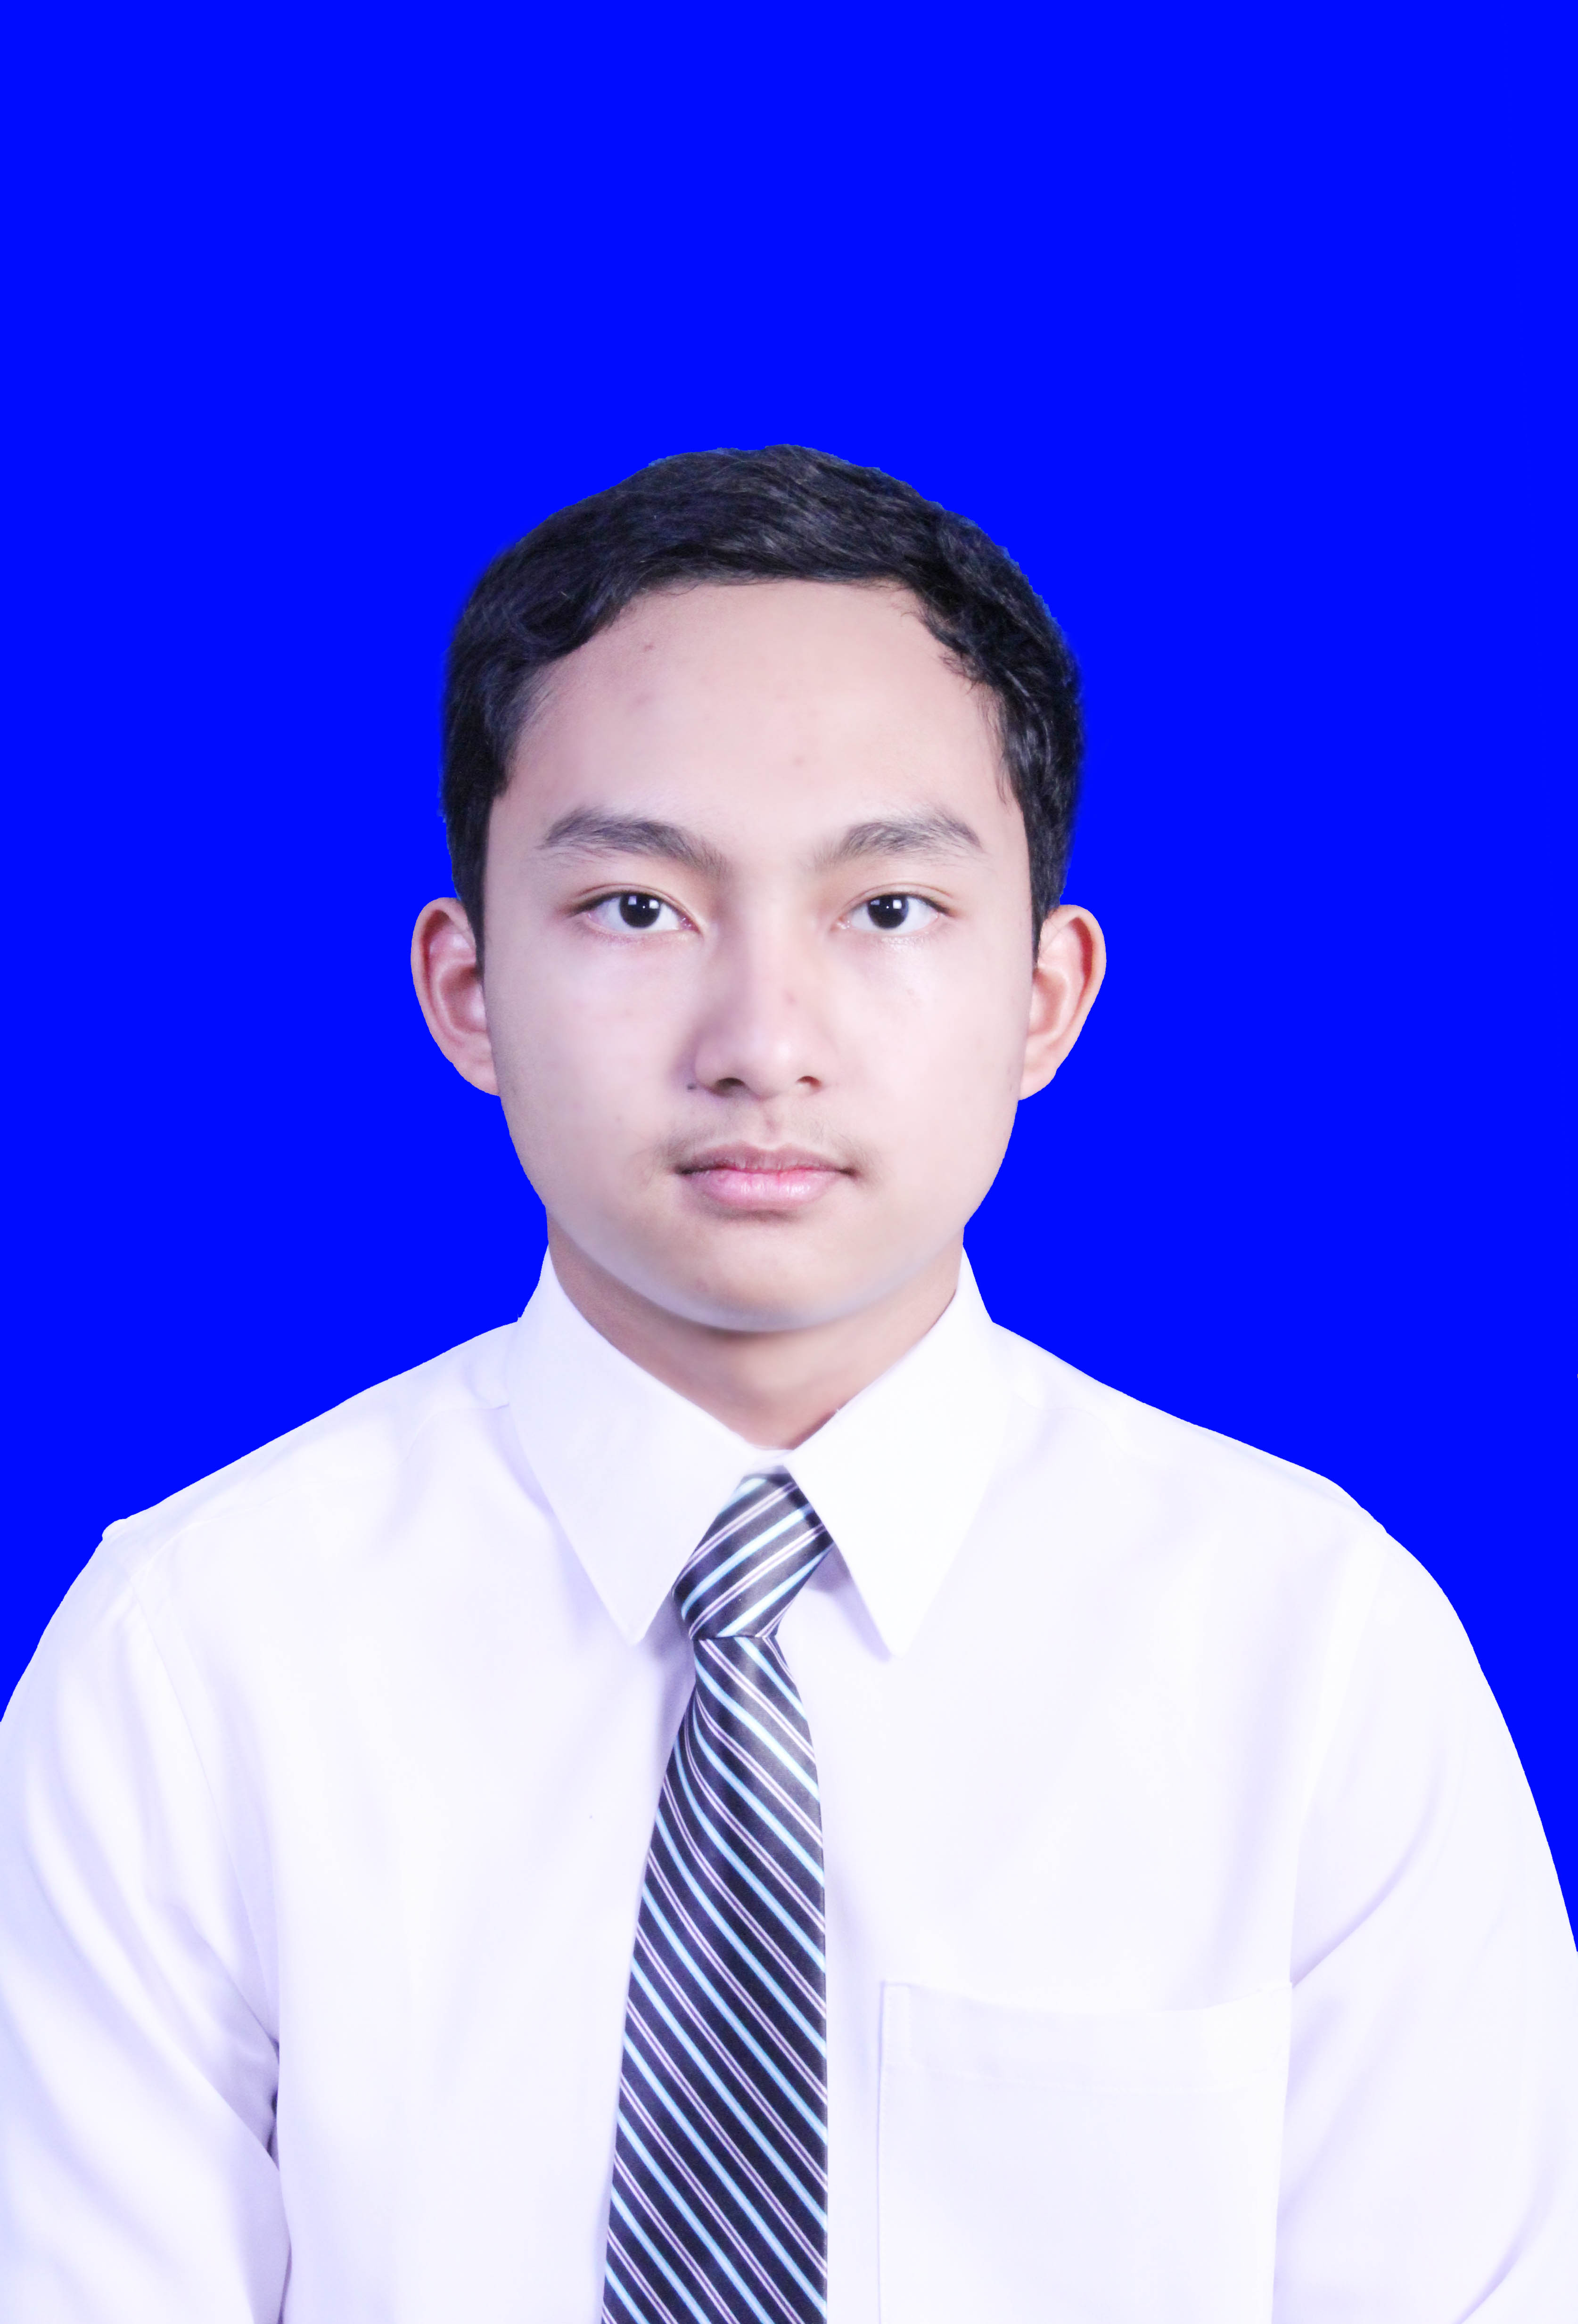
\includegraphics[width=3cm,height=4.5cm]{pasfoto.jpg}}} \\
		{Lampung Selatan, xx xxxx 20xx} & \\
		Penulis, & \\[8ex]
		Dimas Wahyu Saputro   & \\
		{NIM 120450081} & \\[9ex]
	\end{tabular}
\end{table}

\begin{center}
	\begin{tabularx}{\textwidth}{c@{}lXc@{}}%{ccc}
		Pembimbing I & & & Pembimbing II \\ [9ex]
		Nama Pembimbing 1 beserta gelar & & & Nama Pembimbing 2 beserta gelar \\ 
		NIP. xxxxxxxxxx & & & NIP xxxxxxxxxx
	\end{tabularx}
\end{center}

\begin{center}			
	{Disahkan oleh,} 	\\
	{Koordinator Program Studi Sains Data}\\
	{Jurusan Sains} \\
	Institut Teknologi Sumatera\\[9ex]	
	{Nama Koorprodi beserta gelar}\\
	{NIP xxxxxxxxxx}	
\end{center}




